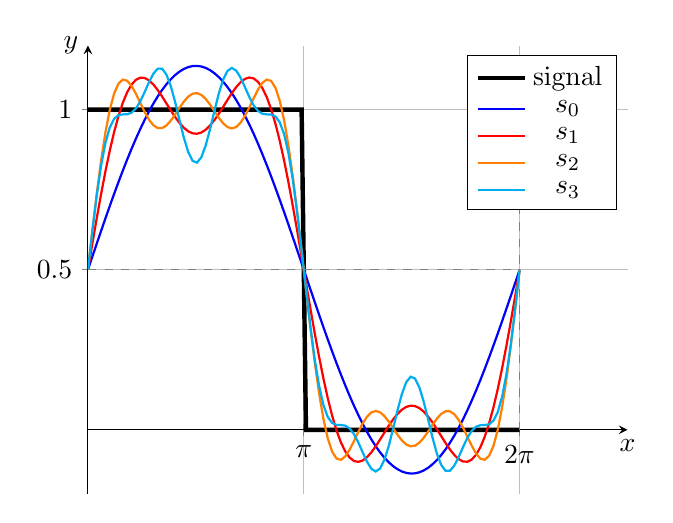
\begin{tikzpicture}
	\begin{axis}[
		xmin = 0, xmax = 2.5 * pi,
		ymin = -0.2, ymax = 1.2,
		domain = 0 : 2 * pi,
		grid=both,
		xlabel = $x$,
		ylabel = $y$,
		axis x line = center, 
		axis y line = center,
		every axis x label/.append style = {below},
		every axis y label/.append style = {left},
		samples = 100,
		xtick = {0, 3.14, 6.28},
		xticklabels = {$0$, $\pi$, $2\pi$},
		declare function = {
		  s(\x) = ifthenelse(\x < pi, 1, 0);
		  s0(\x) = 0.5 + (2 / pi) * sin(deg(\x);
		  s1(\x) = s0(\x) + (2 / pi) * sin(3 * deg(\x)) / 3.0));
		  s2(\x) = s1(\x) + (2 / pi) * sin(5 * deg(\x)) / 5.0));
		  s3(\x) = s1(\x) + (2 / pi) * sin(7 * deg(\x)) / 7.0));
		}, ]
		
		\addplot[ultra thick, black] {s(x)};
		\addplot[thick, blue] {s0(x)};
		\addplot[thick, red] {s1(x)};
		\addplot[thick, orange] {s2(x)};
		\addplot[thick, cyan] {s3(x)};
		\legend{signal, $s_0$, $s_1$, $s_2$, $s_3$};    
		
		% labels
		\draw[gray, dashed] (0, 0.5) -- (2 * pi, 0.5);
		\draw[gray, dashed] (2 * pi, 0) -- (2 * pi, 1);
	\end{axis}
\end{tikzpicture}